\subsection{Połączenie z kontem gry}
		Załóżmy, że użytkownik tej aplikacji będzie chciał wykonać kilka zadań w nadchodzących meczach. W tym celu musi podać nazwę swojego konta po to, aby serwer mógł pobierać odpowiednią historię meczów. Jednak w tym miejscu pojawia się problem. Co, jeśli ktoś poda nazwę nieswojego konta? Będzie wtedy czerpał korzyści z cudzych osiągnięć, a prawowity właściciel nie będzie nic z tego miał. Rozwiązaniem musi być więc potwierdzenie posiadania konta.\par
	\subsubsection{League of Legends}
			Niestety, League of Legends nie posiada takiego mechanizmu. Kuszącą propozycją byłoby pobranie od użytkownika loginu i hasła i zdalne zalogowanie się na jego konto w celu sprawdzenia wiarygodności. Ten pomysł jednak naruszałby zasady bezpieczeństwa. W razie wykrycia, aplikacja zostałaby dożywotnio zablokowana. Innym aspektem jest to, że jeśli jakaś aplikacja prosi o dane logowania na inną domenę, to można z wysokim prawdopodobieństwem założyć, że w ten sposób spróbuje włamać się na te konto.\par
			Innym podejściem byłoby wykonanie określonej czynności, do której tylko właściciel miałby dostęp. Każde konto w League of Legends posiada zbiór stron zwanych \blockquote{Mastery Pages}. Jest to lista maksymalnie 20 stron z ustawieniami gracza, z której każda może zostać nazwana indywidualnie. To, plus fakt, że API udostępnia URI, które zwraca ich całą listę powoduje, że sposób ten stał się rozwiązaniem jak połączyć konto aplikacji z kontem League of Legends.\par
			Po wypełnieniu i wysłaniu formularza (rysunek \ref{img:exampleImage}) serwer sprawdza, czy takie konto istnieje w podanym regionie oraz czy inny użytkownik nie ma przypisanego konta o tej nazwie. W przypadku, gdy obie wersje się potwierdzą, użytkownik zostanie przekierowany na stronę z obecnym statusem (rysunek \ref{img:exampleImage}). Na niej zostanie poinformowany jak musi nazwać jedną ze swoich Mastery Page. Po nazwaniu strony i wciśnięciu przycisku do weryfikacji status konta zostanie zaktualizowany (rysunek \ref{img:exampleImage}).\\
\begin{figure}[!ht]
	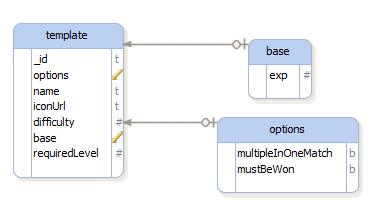
\includegraphics[width=\linewidth]{img/exampleImage}
	\caption{Example caption}
	\label{img:exampleImage}
\end{figure}	